% $Id$
%
\documentclass[11pt]{article}
\usepackage[pdftex]{graphicx}
\usepackage{palatino}
\usepackage{color}
\DeclareGraphicsExtensions{.pdf}
\setlength{\topmargin}{0in}
\setlength{\headheight}{0in}
\setlength{\headsep}{0in}
\setlength{\oddsidemargin}{0in}
\setlength{\evensidemargin}{0in}
\setlength{\textheight}{9in}
\setlength{\textwidth}{6.5in}
\setlength{\parskip}{2ex}
\setlength{\parindent}{0in}
\hyphenpenalty=5000
\tolerance=1000
\hbadness=9999
\sloppy
\pagestyle{plain}
%
\begin{document}

\section*{Implementation experience with the two BPKI models}

Having recently converted my code base to the single-trust-anchor
model Russ recommended, I thought it might be useful to share what
I've learned.  This may not apply to all implementations, but it does
apply to mine, and given what I understand of RIPE's business model,
it will probably apply to RIPE's implementation as well.

In spite of a strong desire to do so, I was not able to use exactly
the same BPKI keys and certificates for HTTPS and CMS.  The reason for
this is simple: each hosted entity in my engine has its own BPKI, as
does the hosting entity, but the HTTPS listener is shared.  The only
ways I know of to avoid this would be to use separate listeners for
each hosted entity, which scales poorly, or to rely on the TLS
``Server Name Indication'' extension (RFC 4366 3.1) which is not yet
widely implemented.

\begin{figure}[hbp]
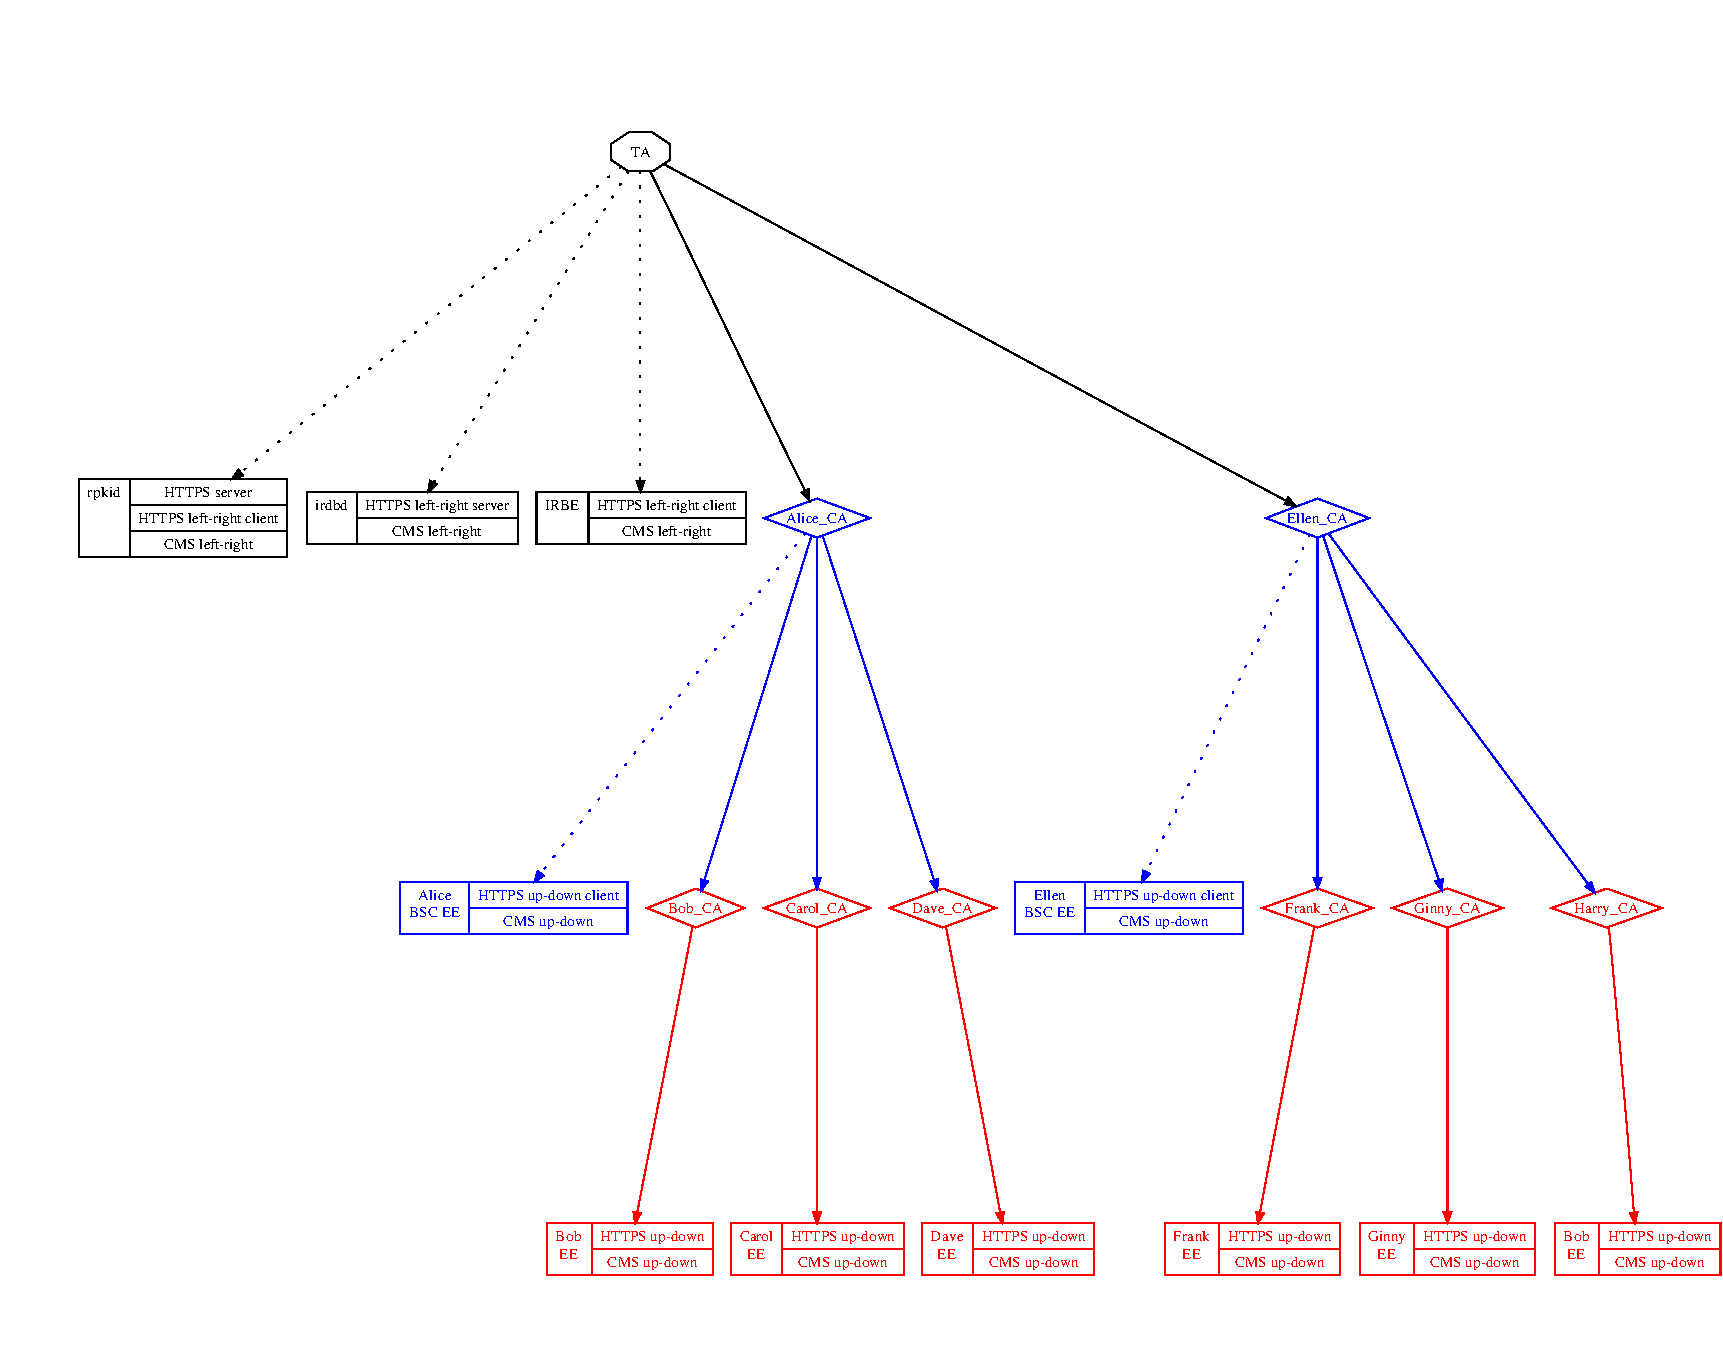
\includegraphics[width = 6.5in]{bpki-symmetric}
\caption{Symmetric BPKI model}
\label{bpki-symmetric}
\end{figure}

Figure \ref{bpki-symmetric} shows my engine's view of the BPKI tree in
the symmetric model.  Black objects belong to the hosting entity, blue
objects belong to the hosted entities, red objects are cross-certified
objects from peers.  The arrows indicate certificate issuance: solid
arrows are the ones that my own RPKI engine will care about during
certificate validation, dotted arrows show the origin of EE
certificates my engine uses to sign things.  ``BSC'' stands for
``business signing context,'' which is a database object in my
implementation representing the context needed to sign a CMS message
or TLS session.

Other than the above-mentioned annoyance with the HTTPS server
certificate, the ``symmetric'' BPKI model worked out pretty much as
expected here.  The certificate tree looks complicated, but the set of
certificates needed to build a particular validation chain is obvious,
again excepting the HTTPS server case, where client certificate is the
first hint that the engine has of the client's identity, so the server
must be prepared to accept any current client certificate.

\begin{figure}[hbp]
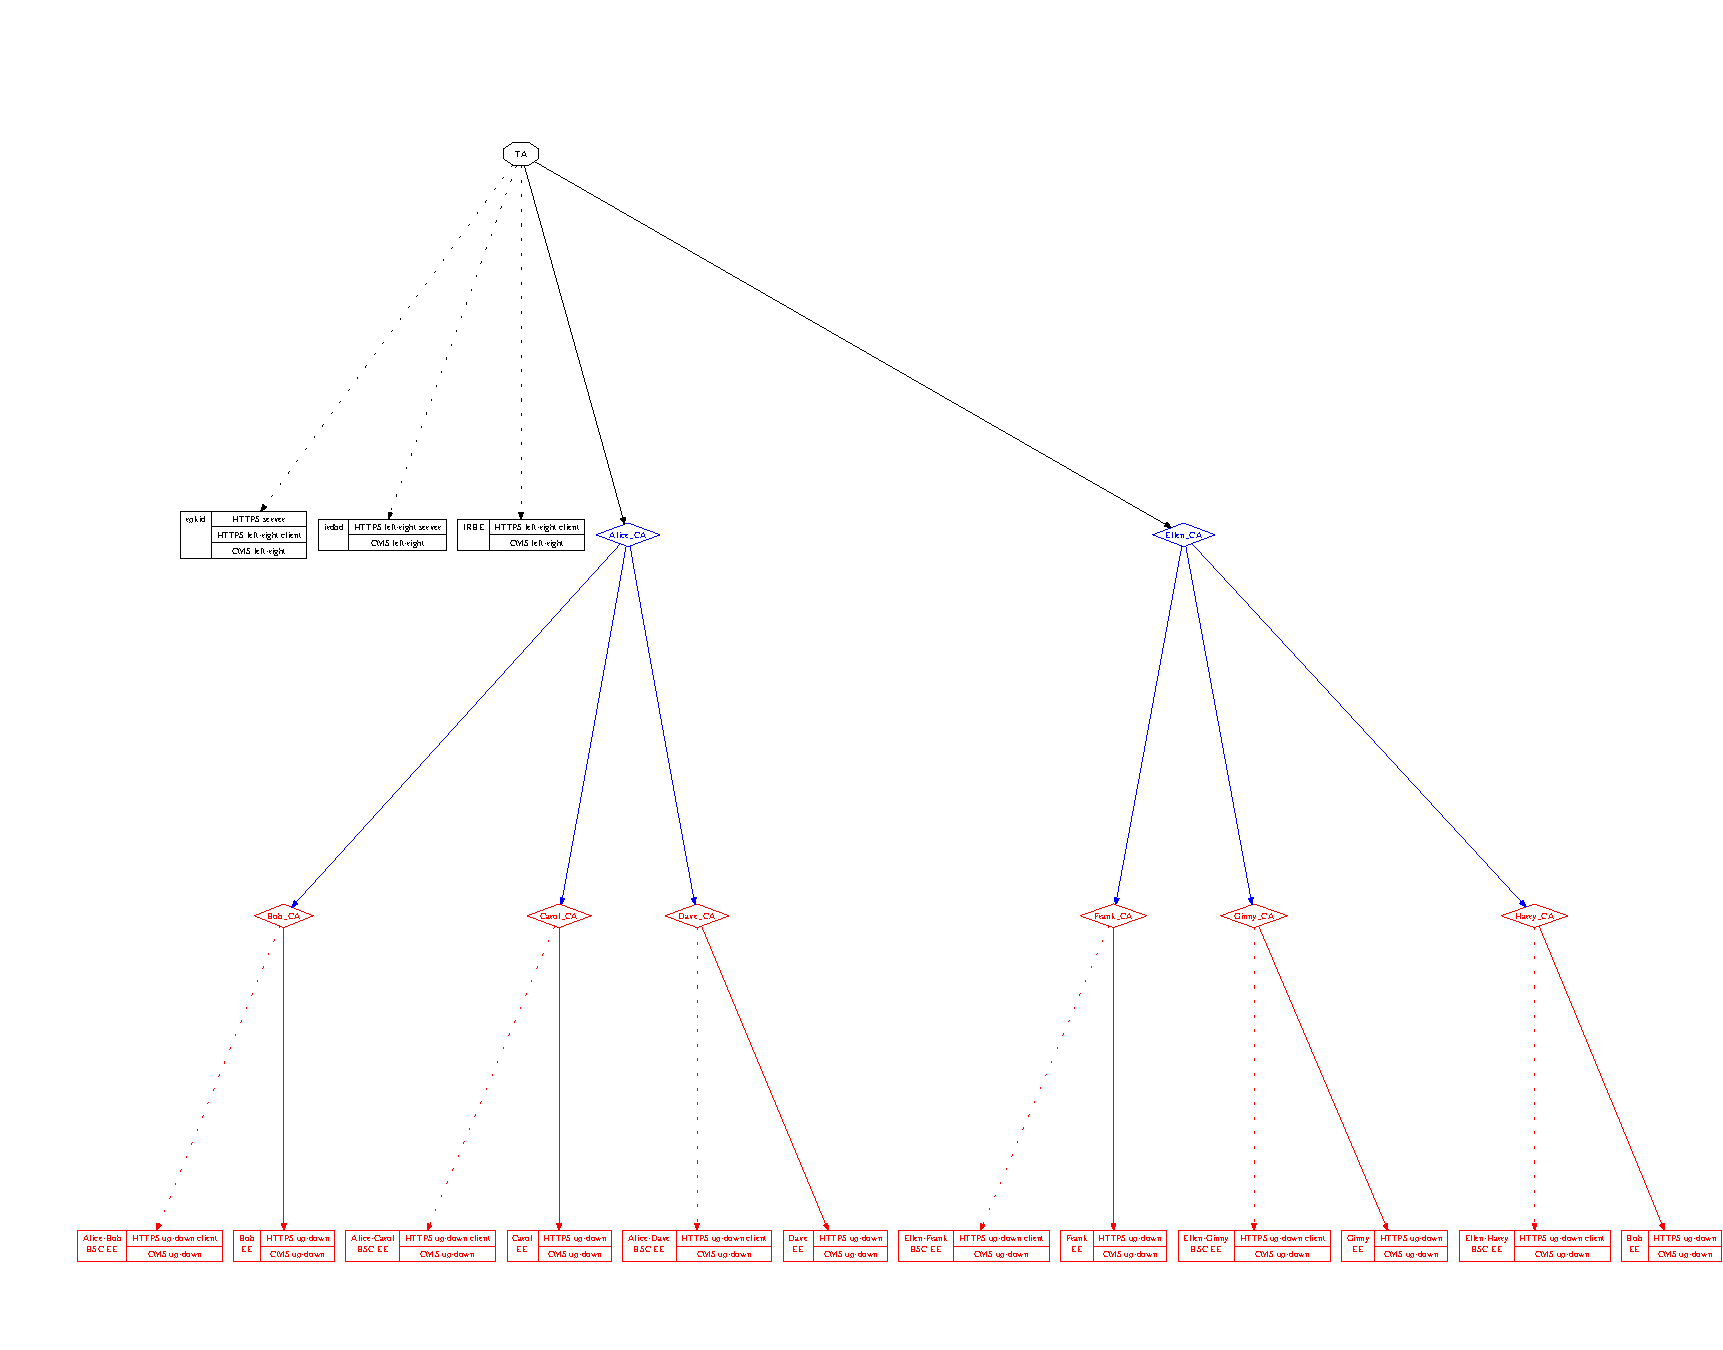
\includegraphics[width = 6.5in]{bpki-asymmetric}
\caption{Asymmetric BPKI model}
\label{bpki-asymmetric}
\end{figure}

Figure \ref{bpki-asymmetric} shows my engine's view of the BPKI tree
in the asymmetric model.  Note that not much has changed here from the
symmetric case.  As far as I can tell, the asymmetric model is just as
complex for my engine as the symmetric model; the only real difference
is that the engine has to keep track of a larger number of BSC EE
certificates in the asymmetric case.

\end{document}
